\chapter{Test e risultati}

Completato lo sviluppo dell'applicazione, ha avuto luogo la fase finale nonché probabilmente la più importante: il testing 
di varie configurazioni e la conseguente raccolta ed analisi dei risultati, al fine di valutare i vantaggi e gli svantaggi di 
un porting sul sistema Android.

A differenza del testing su Raspberry Pi, i cui modelli sono molto standardizzati e distribuiti dallo stesso produttore,
per gli smartphone Android i risultati ottenuti in termini di performance e consumi possono variare anche molto al variare
del dispositivo, a seconda delle caratteristiche tecniche di quest'ultimo.

Per quanto riguarda il seguente progetto, i test sono stati svolti su un dispositivo Android basato sul 
SoC \textit{Qualcomm Snapdragon 730} (sul quale è presente una CPU octa-core).\\

\section{Testing}

Ai fini del testing sono stati utilizzati fotogrammi precedentemente estratti: riprodurre l'intero ciclo di esecuzione OTV
su Android, comprese le fasi di acquisizione ed estrazione introdurrebbe diverse complessità, costringendo a fare i conti con 
diversi problemi (ad esempio, la mancanza di \textit{ffmpeg} su Android).
Difatti, nel testare l'applicazione si è considerata esclusivamente la fase di esecuzione, tralasciando le altre tre fasi
presentate in \autoref{sec:ciclo} principalmente per motivi di tempo. L'esecuzione di OTV rappresenta comunque la fase più
importante e con il maggior numero di variabili che possano influenzare le prestazioni e i consumi: le analisi che ne
conseguono sono sicuramente indicative delle potenzialità di un dispositivo.

Il testing è stato eseguito mediante l'ausilio degli strumenti forniti dalla repository GitHub di OTV (\cite{otvgit}),
in particolare gli script Bash adibiti alla creazione dei file di configurazione richiesti per il funzionamento del programma.
Lo script che implementa l'estrazione dei frame a partire da un file video fa uso del programma
\textit{ffmpeg} e salva i fotogrammi estratti all'interno di una cartella \texttt{frames} il cui percorso va specificato.

La cartella dei frames e gli altri file necessari sono stati quindi prima generati sulla macchina utilizzata per lo sviluppo
dell'applicazione, poi trasferiti sul dispositivo Android mediante l'interfaccia grafica fornita da Android Studio.
Collegando infatti lo smartphone al PC su cui esegue Android Studio è possibile accedere ad una sezione dedicata al file system
del dispositivo.

Come già menzionato, tutti i file di servizio sono stati inseriti all'interno della cartella \texttt{/data/data/\{package\_applicazione\}}
poiché questa fa parte del cosiddetto storage \emph{interno} dell'applicazione, in cui gli accessi non sono vincolati da permessi
richiesti all'utente. Questa cartella inoltre non è accessibile dall'utente se non tramite strumenti esterni al dispositivo 
(come il debugger Android) e può quindi essere utile ad evitare cancellazioni e/o modifiche accidentali dei file necessari.

Particolare attenzione va posta al file \texttt{info\_video.txt}, generato in seguito all'estrazione dei frame. Il file si
presenta nel seguente modo:

\begin{verbatim}
    FPS 25
    Width 715
    Height 540
    FileCount 500
    DirectoryFrame /data/data/gullp.androidotv/frames
    Jump 2
\end{verbatim}

dove il parametro DirectoryFrame rappresenta la directory in cui sono presenti i frame: il file viene letto dall'applicazione
in fase di inizializzazione, quindi è importante che il percorso di tale directory sia accurato.
Tuttavia, essendo il file \texttt{info\_video.txt} generato da uno script eseguito su una macchina differente, è necessario
andare a modificare tale parametro specificando la corrispettiva cartella nel dispositivo Android.

\vspace{1em}

Il processo di testing è avvenuto seguendo un'iterazione di questo tipo:

\begin{enumerate}
    \item Copia delle librerie dinamiche precompilate di OpenCV all'interno del progetto, ottenute con la cross-compilazione 
    e nelle quali è attivo uno specifico set di ottimizzazioni;
    \item Esecuzione dell'applicazione e trascrizione dei risultati ottenuti
    \item Ripetizione del punto 2 fino ad ottenere una quantità soddisfacente di risultati
    \item Reiterazione a partire dal punto 1 utilizzando una nuova configurazione di OpenCV
\end{enumerate}

\vspace{1em}

I risultati così ottenuti sono poi stati sottoposti ad un'analisi finale per stabilire i vantaggi di ciascuna configurazione. 

\section{Stima dei consumi energetici}
\label{sec:stimaconsumi}

Data l'influenza che i consumi energetici hanno sulla realizzabilità e sulla valutazione di un dispositivo embedded di questo
tipo, si è deciso di svolgere --- anche se non approfonditamente --- una stima dell'energia consumata da esso.
È importante notare che si tratta di una stima, poiché gli strumenti utilizzati consentono un livello di precisione piuttosto
basso nella misurazione dei consumi su periodi piuttosto brevi di tempo.

Per stimare i consumi energetici dell'esecuzione di OTV è stato utilizzato uno strumento messo a disposizione per gli 
sviluppatori Android: \textit{\textbf{Battery Historian}}. Si tratta di un tool web il cui utilizzo molto semplice è 
descritto in \cite{adev_battery}. In sostanza, analizza i file di log generati dal dispositivo e ne visualizza gli eventi
correlati al consumo di batteria, fornendone una presentazione ad alto livello tramite grafici e tabelle.
Tra i parametri analizzati da Battery Historian figurano il livello di carica della batteria (in $mAh$) e la tensione generata
da essa (in $mV$). L'analisi viene svolta su tutto l'arco temporale coperto dai log: è bene quindi resettare i log relativi
all'uso della batteria.

I file di log necessari all'utilizzo di Battery Historian possono essere acquisiti mediante il debugger Android (\texttt{adb}): 
la procedura guidata è disponibile in \cite{adev_batlog}.

\begin{figure}[h!]
    \begin{center}
        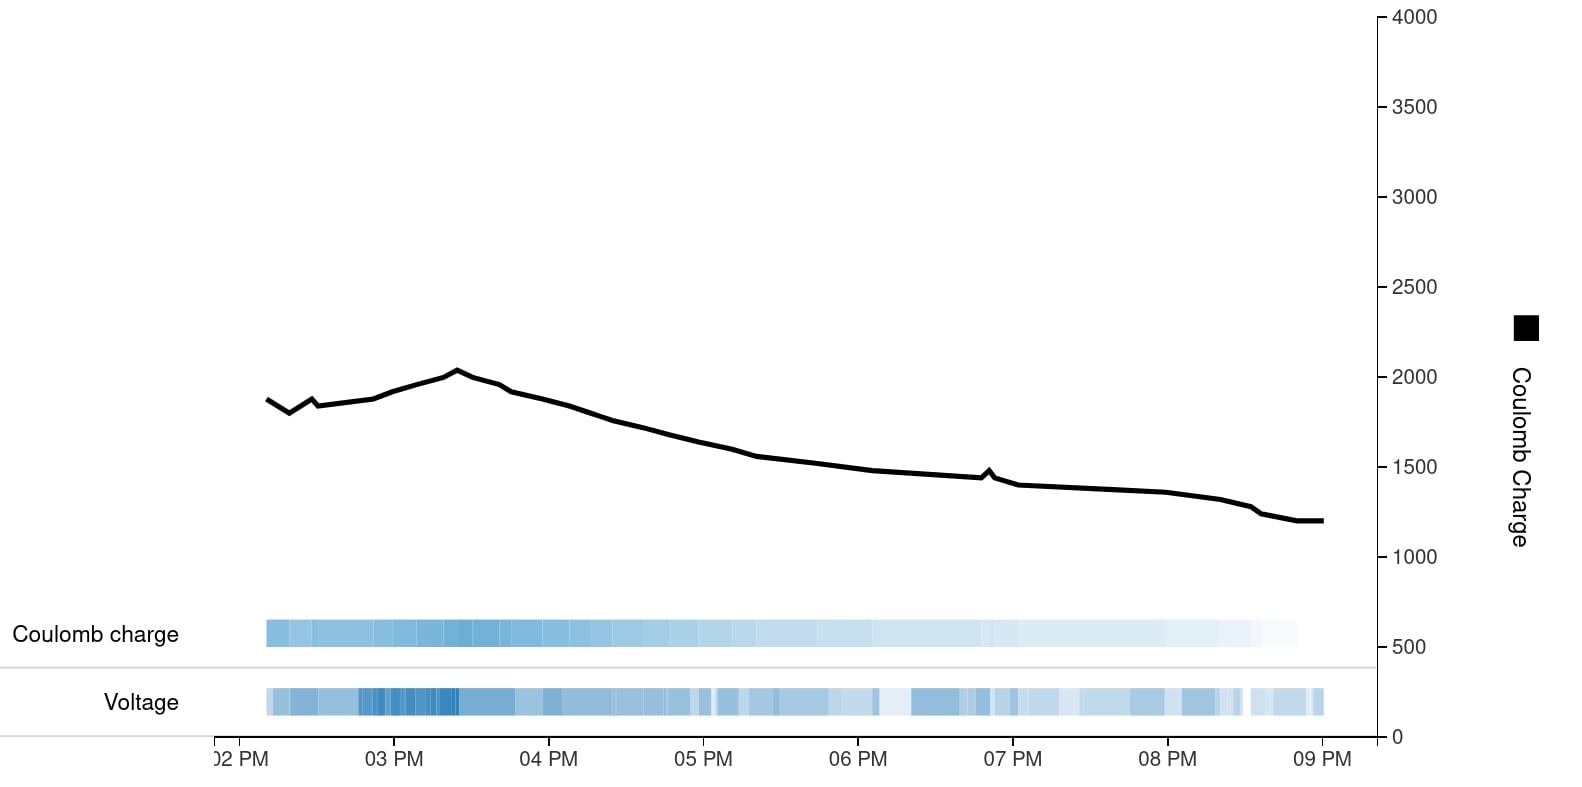
\includegraphics[scale=0.28]{img/battery_historian_coulomb.jpg}
        \caption{Andamento nel tempo del livello di carica della batteria in $mAh$}
    \end{center}
\end{figure}

L'immagine di cui sopra rappresenta uno dei grafici ottenibili con Battery Historian di maggiore interesse al fine di
determinare il consumo energetico: l'andamento del livello di carica. Passando il cursore lungo il grafico è possibile
ottenere informazioni aggiuntive particolarmente utili.

\begin{figure}[h!]
    \begin{center}
        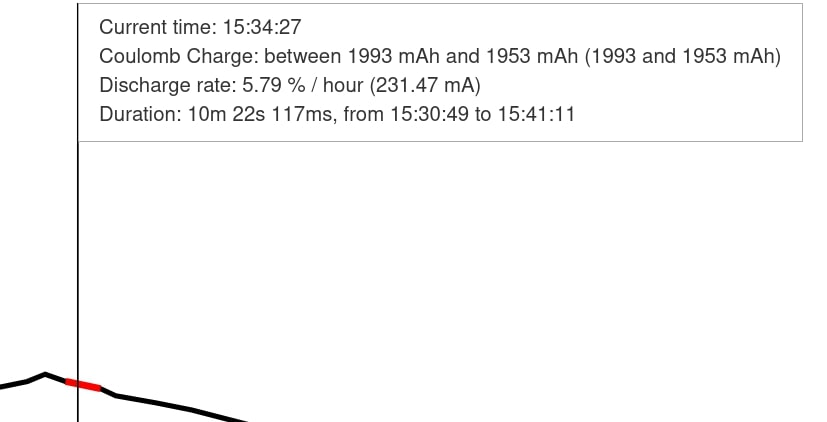
\includegraphics[scale=0.35]{img/battery_historian_hover.jpg}
        \caption{Informazioni dettagliate relative ad uno specifico intervallo di tempo}
    \end{center}
\end{figure}

Come si può in parte notare dalla figura, l'andamento è discretizzato con dei campionamenti del livello di carica ad 
intervalli di tempo non regolari.

Il dettaglio più interessante tra quelli forniti è il \textit{Discharge rate} espresso in $mA$: è il rapporto tra la differenza
di carica $\Delta Q$ e la lunghezza dell'intervallo $\Delta t$ e rappresenta quindi la media della \textbf{corrente in uscita} 
dalla batteria sull'intervallo di tempo:

\begin{equation*}
    I_{i} = \frac{\Delta Q_i}{\Delta t_i}
\end{equation*}

È possibile comunque applicare la medesima espressione conoscendo la carica in $mAh$ sapendo che $1~mAh = 3.6~C$.

A questo punto, per calcolare la potenza dissipata dallo smartphone durante l'esecuzione di OTV e dunque ottenere l'energia 
consumata, è necessario avere a disposizione altre due informazioni:
\begin{itemize}
    \item I tempi di inizio e fine dell'esecuzione di OTV
    \item Il valore della tensione durante l'esecuzione
\end{itemize}

Entrambe le informazioni sono reperibili immediatamente grazie alle tabelle fornite da Battery Historian.
Analizzando i grafici della tensione si nota che essa non è costante ma soggetta a variazioni molto frequenti, 
tende tuttavia ad assumere valori piuttosto omogenei con una bassa varianza ed è quindi approssimabile ad un valore medio
con una discreta precisione, specie se l'intervallo di tempo analizzato è relativamente piccolo (60 secondi con la configurazione
peggiore di OTV).\\
Supponendo quindi di approssimare la tensione ad un valore $V$ e di avere a disposizione $N$ intervalli di calcolo della
corrente durante l'esecuzione di OTV, è possibile calcolare l'energia consumata basandosi sulla potenza media dissipata come segue:

\begin{equation*}
    E = P \cdot \Delta t = \sum_{i = 1}^{N}~V I_i \cdot \Delta t_i
\end{equation*}

Dove $\Delta t$ è la durata dell'esecuzione di OTV e $\Delta t_i$ è la lunghezza dell'intervallo di tempo in cui
si verifica la corrente i-esima $I_i$.\\
Poiché, come fatto notare poco sopra, l'esecuzione di OTV termina in un lasso di tempo piuttosto breve, sono spesso osservabili
tensioni e correnti costanti lungo tale periodo.

\section{Analisi dei risultati}

Al termine del progetto ha avuto luogo la fase di analisi dei risultati, sia dal punto di vista delle prestazioni che dei 
consumi. Tutti i test sono stati eseguiti sullo stesso campione video della durata di 20 secondi. La maggior parte dei test
è stata eseguita con fotogrammi ad \textit{Half Resolution} in quanto, alla luce dei risultati ottenuti in \cite{app11157027},
questa configurazione si è dimostrata il migliore compromesso tra affidabilità dei risultati e velocità di esecuzione. Per lo
stesso motivo, nessun test è stato svolto con una configurazione a \textit{Quarter Resolution}.

L'ottimizzazione relativa all'utilizzo della GPU è stata esclusa dai test poiché, dopo alcuni tentativi, è stato impossibile
abilitarla correttamente: analizzando i log del sistema Android, si riscontrano errori di permessi e di letture relativi alla
GPU del dispositivo, probabilmente dovuti ad un mancato supporto di OpenCL.

Si riportano di seguito i dati ottenuti in termini di tempo di esecuzione, evidenziando le differenze tra le varie configurazioni.
I tempi riportati corrispondono al valore medio del tempo di esecuzione osservato tra tutti i test svolti, la varianza è 
risultata tale da essere trascurabile.

\begin{figure}[h!]
    \begin{center}
        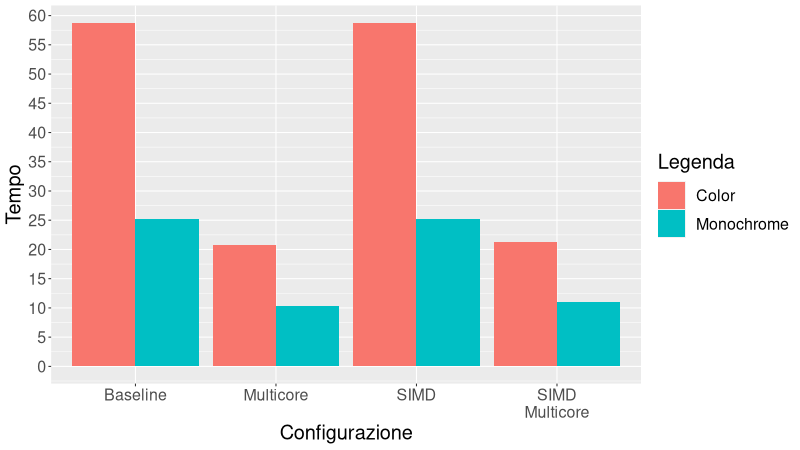
\includegraphics[scale=0.45]{img/execution_time.png}
        \caption{Tempo di esecuzione [s] (\textbf{Half Resolution})}
        \label{fig:execution_time}
    \end{center}
\end{figure}

Come si può notare in \autoref{fig:execution_time}, l'elaborazione in scala di grigi influisce notevolmente sulle prestazioni, riducendo almeno del 50\% i tempi
in tutti i test svolti. Sorprendentemente, l'abilitazione di istruzioni SIMD NEON non ha influito in alcun modo 
sull'esecuzione, risultando anzi in un lieve peggioramento delle prestazioni (pochi decimi di secondo). Il motivo di ciò non è
ben chiaro e potrebbe essere riconducibile a diverse cause, ad esempio un banale errore di configurazione.

\newpage

Nel testare invece i consumi energetici sono state abilitate tutte le possibili ottimizzazioni software fornite dal sistema 
Android: disabilitazione di connessione dati, Wi-Fi, Bluetooth, attivazione della \textbf{modalità risparmio energetico} e
luminosità dello schermo impostata al minimo, avendo cura di mantenere attive le funzionalità basilari necessarie alla comunicazione (es. SMS). Nessuna di queste 
ottimizzazioni ha influito negativamente sulle prestazioni dell'applicazione.

\begin{figure}[h!]
    \begin{center}
        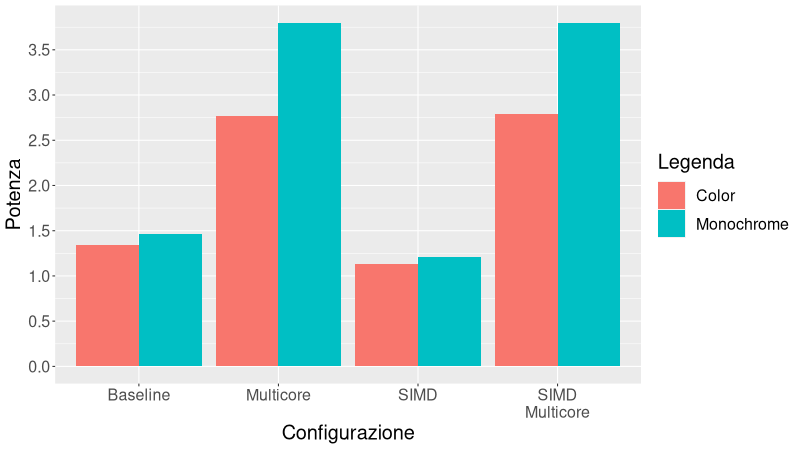
\includegraphics[scale=0.45]{img/power.png}
        \caption{Potenza dissipata [W] (\textbf{Half Resolution})}
        \label{fig:power}
    \end{center}
\end{figure}

\begin{figure}[h!]
    \begin{center}
        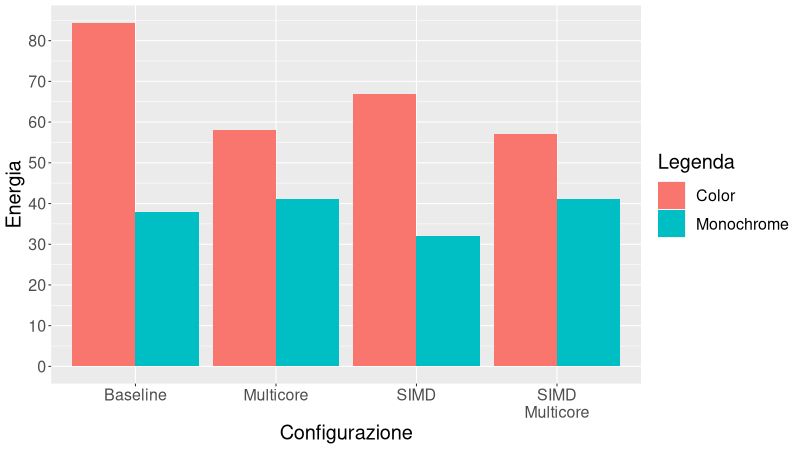
\includegraphics[scale=0.45]{img/energy.png}
        \caption{Energia consumata [J] (\textbf{Half Resolution})}
    \end{center}
\end{figure}

Contrariamente a quanto riscontrato con i test su Raspberry Pi, la configurazione che pare garantire il minor consumo di energia
sembra essere quella che fa uso del minor numero di ottimizzazioni hardware. Si ricorda che i grafici di potenza ed energia
qui riportati sono una stima dei consumi energetici ottenuti con il metodo descritto in \autoref{sec:stimaconsumi}, 
il consumo reale potrebbe discostarsi da quello stimato.\\
Risultano in effetti insoliti i picchi di potenza in \autoref{fig:power} registrati con configurazioni \textit{Multicore} in elaborazioni monocromatiche.

Confrontando queste stime con i consumi dei dispositivi Raspberry Pi riportati in \cite{app11157027}, si nota un netto miglioramento
dei consumi energetici stimati. Questa analisi va comunque corredata da considerazioni più complete circa il ciclo di esecuzione
dell'applicazione Android finale.